\documentclass{article}
\usepackage[utf8]{inputenc}
\usepackage{hyperref}
\usepackage{graphicx}

\begin{document}
\section{Description of the developed functionalities}
\subsection{Scenario Editor}

The Scenario Editor (Figure 1) is a new feature with which a configuration file can be created, opened, modified, saved and exported to mas2g. The editor can be divided into two main parts: The configuration panel and the entity panel.
In the toolbar there is a button "File". When clicked a drop down menu will appear with the options to open, create, save and export the file. Exiting the editor is also possible here.

\begin{figure}[h]
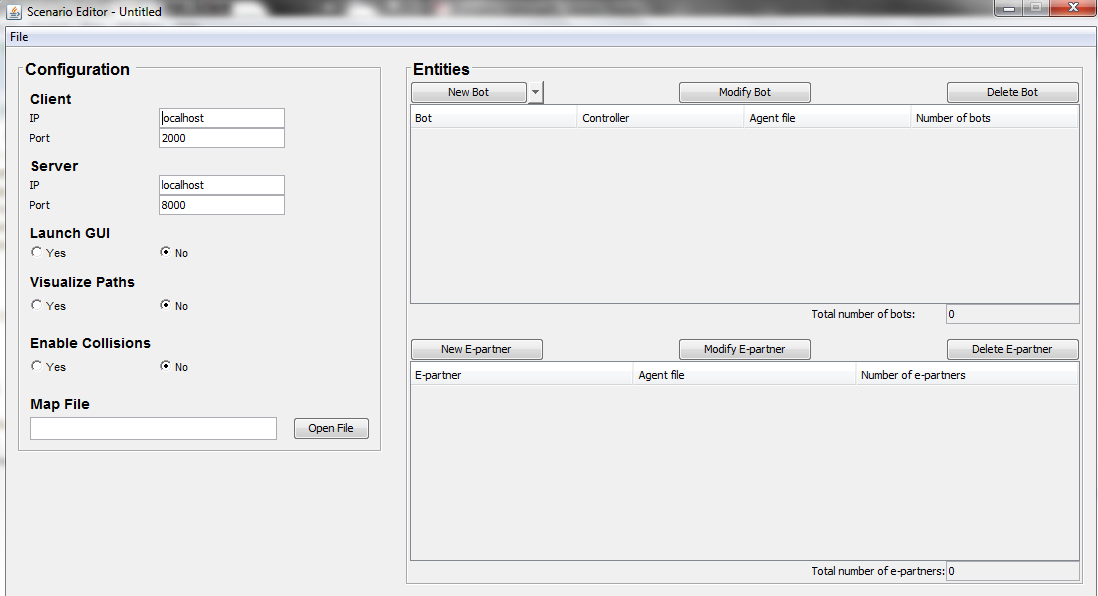
\includegraphics[width=\textwidth]{scenario-editor.png}
\caption{Scenario Editor}
\end{figure}

\subsection{Configuration panel}
Here the client IP, client port, server IP and server port can be set. Also whether the GUI needs to be launched, whether the paths will be visualized and whether collisions will be enabled can be set here. Lastly, selecting a map file to use in the configuration is possible.

\subsection{Entity Panel}
The bots can be created, modified and deleted here with the following three buttons: "New bot", "Modify bot" and "Delete bot". Next to the "New bot" button there is a dropdown button. Here you can add a new default bot to the bot list, which is being displayed below these three buttons. On the right side, under the bot list, the total number of bots is shown.

Below this, there are the three e-partner buttons, followed by the e-partner list and the total amount of e-partners created. It has the same functionalities as the bots part, but then for the e-partner.

By selecting a bot or e-partner and then clicking on the modify bot or e-partner button, the Bot Store or E-partner Store will open. Here you can further configure your bot or e-partner.

\subsection{Human Player GUI}

One of the functionalities we have extended is the Human Player GUI (Figure 2). We roughly splitted the interface up in two sections. The map is being displayed on the left, while the chat sessions are being displayed on the right.

\begin{figure}[h]
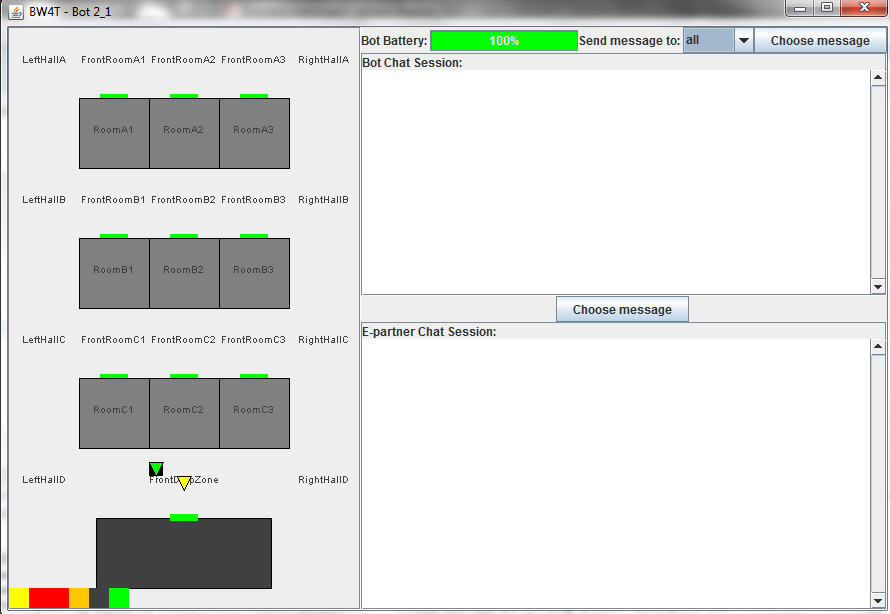
\includegraphics[width=\textwidth]{hpg.png}
\caption{Human Player GUI}
\end{figure}

\subsection{The map}
In the map there is the possibility to zoom in and zoom out with the mouse scrollbutton. There is also a scrollbar, which will appear when the map is larger than the area where the map is being displayed. Upon clicking on the rooms, corridors, blocks and/or e-partners, a dropdown menu will appear with the possible actions.

\subsection{Chat sessions}
Originally there was only one chat session, but because of the addition of the e-partners, we have decided to split up the chat session into two chat sessions. One for bots to bots and one for bot to e-partner.

The bot battery is being displayed first. Next to it, there is a dropdown box where the user can select to which agent he/she wants to send a message to. There is also a button: "send message", where you can select the message to send. Below this, there is the chat session box of the bots. A dropdown menu with possible answers to questions will appear when clicked in the box. \\

Some space is reserved for the e-partner chat session and message button below the bot chat sessions. These will only appear when an e-partner is being held by the bot. As soon as the e-partner is dropped, the message button of the e-partner will be disabled. The chat box will not disappear though. This way the e-partner can still send messages to the bot, if it has gps enabled. The message button is only used for sending messages to the e-partner and dropping the e-partner.


\end{document}